\documentclass[tikz, border=10pt]{standalone}

\usepackage{tikz}
\usetikzlibrary{positioning, arrows.meta}

% ==============================================================================
% Styles
% ==============================================================================
\tikzset{
  topbox/.style={
    rectangle, rounded corners,
    draw=blue!60!black, fill=blue!15,
    thick, text centered,
    text width=4.6cm, minimum height=1.2cm
  },
  root/.style={
    rectangle, rounded corners,
    draw=red!70!black, fill=red!12,
    very thick, text centered,
    text width=10cm, minimum height=1.4cm
  },
  group/.style={
    rectangle, rounded corners,
    draw=blue!60!black, fill=blue!10,
    thick, text centered,
    text width=4.8cm, minimum height=1.1cm
  },
  project/.style={
    rectangle, rounded corners=2pt,
    draw=gray!60, fill=gray!10,
    thick, align=left,
    text width=5.6cm,   % <-- reduced
    minimum height=0.8cm % <-- reduced
  },
  arrow/.style={thick, -{Stealth[length=3mm]}}
}

\begin{document}
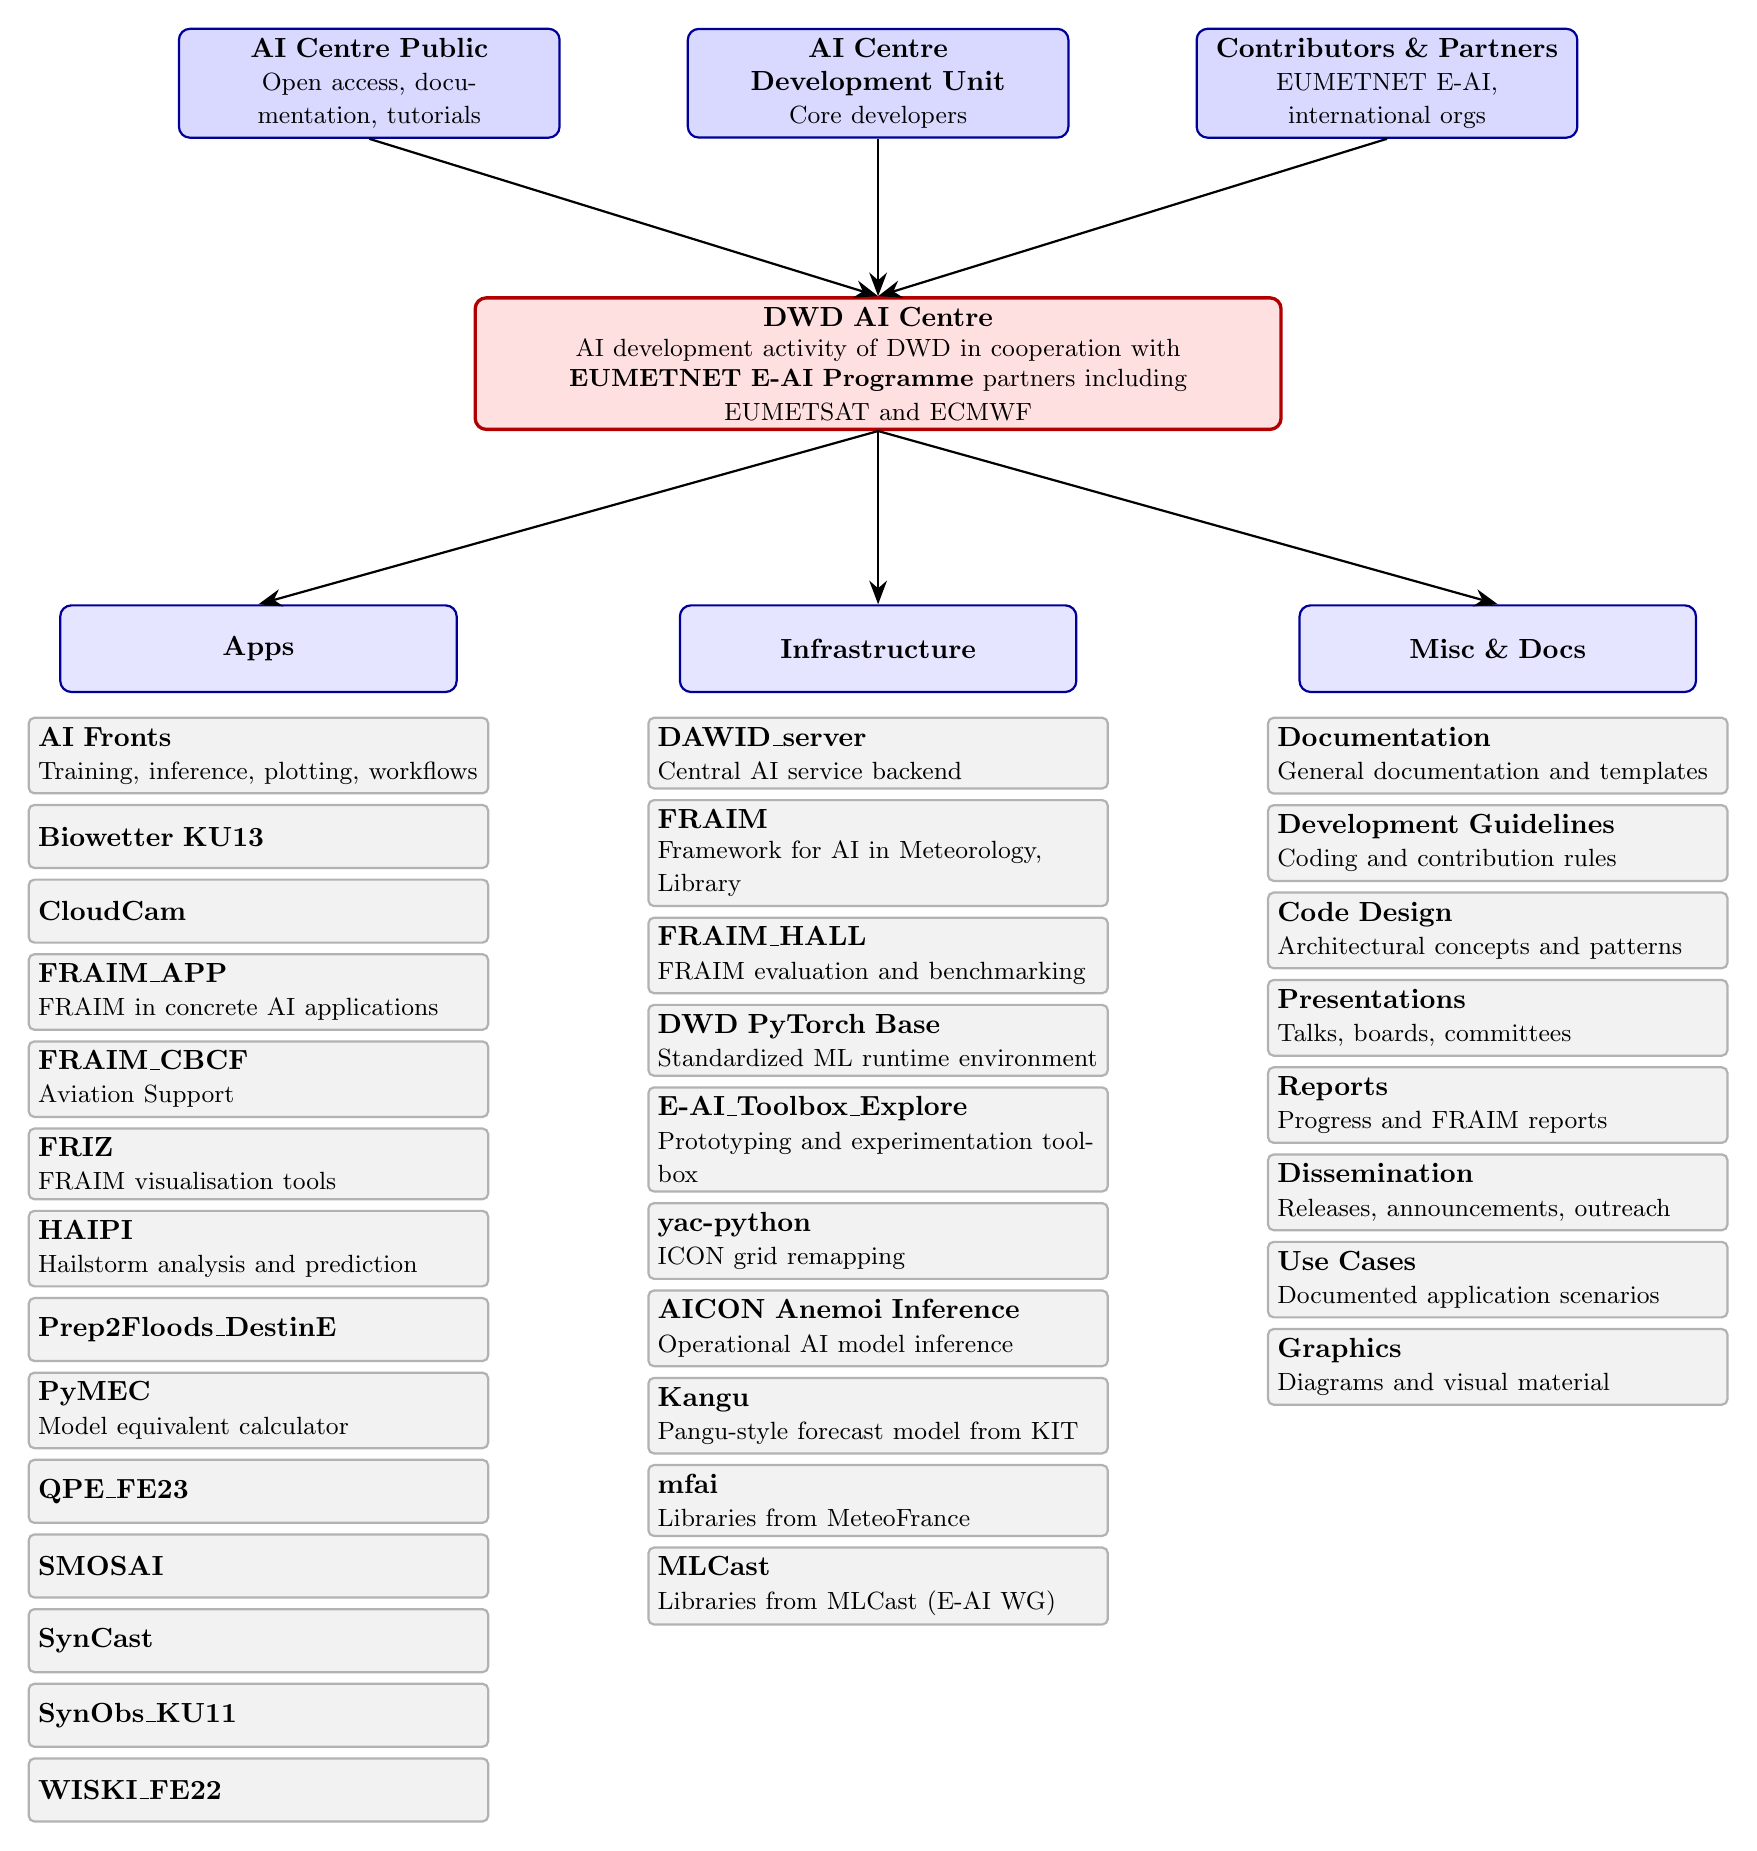
\begin{tikzpicture}[node distance=0.45cm]

% ==============================================================================
% Top access / people level
% ==============================================================================
\node[topbox] (public) {
  \textbf{AI Centre Public}\\
  \small Open access, documentation, tutorials
};

\node[topbox, right=1.6cm of public] (devunit) {
  \textbf{AI Centre \\Development Unit}\\
  \small Core developers
};

\node[topbox, right=1.6cm of devunit] (partners) {
  \textbf{Contributors \& Partners}\\
  \small EUMETNET E-AI, international orgs
};

% ==============================================================================
% Root
% ==============================================================================
\node[root, below=2.0cm of devunit] (root) {
  \textbf{DWD AI Centre}\\
  \small AI development activity of DWD in cooperation with\\
  \small \textbf{EUMETNET E-AI Programme} partners including \\
  \small EUMETSAT and ECMWF
};

% ==============================================================================
% APPS
% ==============================================================================
\node[group, below left=2.2cm and 0.2cm of root] (apps) {
  \textbf{Apps}
};

\node[project, below=0.3cm of apps] (a1) {
  \textbf{AI Fronts}\\
  \small Training, inference, plotting, workflows
};

\node[project, below=0.12cm of a1] (a2) {
  \textbf{Biowetter KU13}
};

\node[project, below=0.12cm of a2] (a3) {
  \textbf{CloudCam}
};

\node[project, below=0.12cm of a3] (a4) {
  \textbf{FRAIM\_APP}\\
  \small FRAIM in concrete AI applications
};

\node[project, below=0.12cm of a4] (a5) {
  \textbf{FRAIM\_CBCF}\\
  \small Aviation Support
};

\node[project, below=0.12cm of a5] (a6) {
  \textbf{FRIZ}\\
  \small FRAIM visualisation tools
};

\node[project, below=0.12cm of a6] (a7) {
  \textbf{HAIPI}\\
  \small Hailstorm analysis and prediction
};

\node[project, below=0.12cm of a7] (a8) {
  \textbf{Prep2Floods\_DestinE}
};

\node[project, below=0.12cm of a8] (a9) {
  \textbf{PyMEC}\\
  \small Model equivalent calculator
};

\node[project, below=0.12cm of a9] (a10) {
  \textbf{QPE\_FE23}
};

\node[project, below=0.12cm of a10] (a11) {
  \textbf{SMOSAI}
};

\node[project, below=0.12cm of a11] (a12) {
  \textbf{SynCast}
};

\node[project, below=0.12cm of a12] (a13) {
  \textbf{SynObs\_KU11}
};

\node[project, below=0.12cm of a13] (a14) {
  \textbf{WISKI\_FE22}
};

% ==============================================================================
% INFRASTRUCTURE
% ==============================================================================
\node[group, below=2.2cm of root] (infra) {
  \textbf{Infrastructure}
};

\node[project, below=0.3cm of infra] (i1) {
  \textbf{DAWID\_server}\\
  \small Central AI service backend
};

\node[project, below=0.12cm of i1] (i2) {
  \textbf{FRAIM}\\
  \small Framework for AI in Meteorology, \\
  \small Library
};

\node[project, below=0.12cm of i2] (i3) {
  \textbf{FRAIM\_HALL}\\
  \small FRAIM evaluation and benchmarking
};

\node[project, below=0.12cm of i3] (i4) {
  \textbf{DWD PyTorch Base}\\
  \small Standardized ML runtime environment
};

\node[project, below=0.12cm of i4] (i5) {
  \textbf{E-AI\_Toolbox\_Explore}\\
  \small Prototyping and experimentation toolbox
};

\node[project, below=0.12cm of i5] (i6) {
  \textbf{yac-python}\\
  \small ICON grid remapping
};

\node[project, below=0.12cm of i6] (i7) {
  \textbf{AICON Anemoi Inference}\\
  \small Operational AI model inference
};

\node[project, below=0.12cm of i7] (i8) {
  \textbf{Kangu}\\
  \small Pangu-style forecast model from KIT
};

\node[project, below=0.12cm of i8] (i9) {
  \textbf{mfai}\\
  \small Libraries from MeteoFrance
};

\node[project, below=0.12cm of i9] (i10) {
  \textbf{MLCast}\\
  \small Libraries from MLCast (E-AI WG)
};

% ==============================================================================
% MISC & DOCS
% ==============================================================================
\node[group, below right=2.2cm and 0.2cm of root] (docs) {
  \textbf{Misc \& Docs}
};

\node[project, below=0.3cm of docs] (d1) {
  \textbf{Documentation}\\
  \small General documentation and templates
};

\node[project, below=0.12cm of d1] (d2) {
  \textbf{Development Guidelines}\\
  \small Coding and contribution rules
};

\node[project, below=0.12cm of d2] (d3) {
  \textbf{Code Design}\\
  \small Architectural concepts and patterns
};

\node[project, below=0.12cm of d3] (d4) {
  \textbf{Presentations}\\
  \small Talks, boards, committees
};

\node[project, below=0.12cm of d4] (d5) {
  \textbf{Reports}\\
  \small Progress and FRAIM reports
};

\node[project, below=0.12cm of d5] (d6) {
  \textbf{Dissemination}\\
  \small Releases, announcements, outreach
};

\node[project, below=0.12cm of d6] (d7) {
  \textbf{Use Cases}\\
  \small Documented application scenarios
};

\node[project, below=0.12cm of d7] (d8) {
  \textbf{Graphics}\\
  \small Diagrams and visual material
};

% ==============================================================================
% Arrows
% ==============================================================================
\draw[arrow] (public.south) -- (root.north);
\draw[arrow] (devunit.south) -- (root.north);
\draw[arrow] (partners.south) -- (root.north);

\draw[arrow] (root.south) -- (apps.north);
\draw[arrow] (root.south) -- (infra.north);
\draw[arrow] (root.south) -- (docs.north);

\end{tikzpicture}
\end{document}
